\subsection{Angular Loss}

\begin{frame}{Назад к классификации}

Ещё раз про классификацию из дескриптора:
\[
\sigma_i(W^\Tr_i d + b_i) = \frac{\exp ( W^\Tr_i d + b_i )}{\sum_j \exp ( W^\Tr_j d + b_j )}
\]

Если мы отнормируем дескиптор $d$ и столбцы $W$, то скалярное произведение внутри экспоненты можно переписать:

\[
\frac{\exp ( \|W_i\|_2 \|d\|_2 \cos \theta_{i} + b_i )}{\sum_j \exp ( \|W_j\|_2 \|d\|_2 \cos \theta_{j} + b_j )} = \{ \|d\|_2 = 1,\, \|W_i\|_2 = 1 \} = 
\frac{\exp ( \cos \theta_{i} + b_i )}{\sum_j \exp ( \cos \theta_{j} + b_j )}
\]

В этом случае мы уменьшаем непосредственно угол между дескриптором и нужным столбцом матрицы $W$.
    
\end{frame}

\begin{frame}{Angular Loss}

А что если нам идею с зазором добавить в оптимизируемый нами угол?
\[
AngularLoss : \frac{e^{ m_1 \cos (m_2 \theta_{i} + m_3)} }{e^{ m_1 \cos (m_2 \theta_{i} + m_3) } + \sum_{j \neq i} e^{ m_1 \cos \theta_{j}} }
\]

\centering
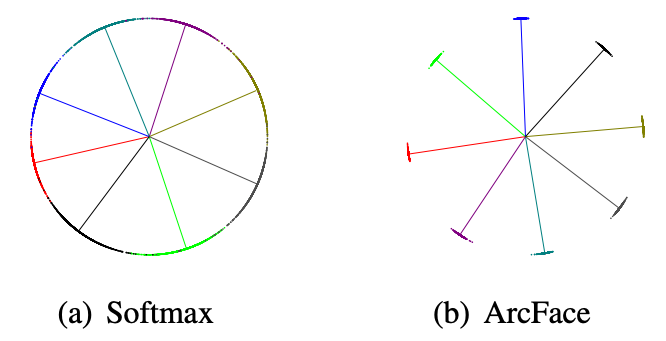
\includegraphics[width=0.5\textwidth]{images/arcface.png}
    
\end{frame}
